%\documentclass{article}
\documentclass[]{article}
\usepackage{bm}
\usepackage{amsmath}
\usepackage{amsfonts}
\usepackage{natbib}
\usepackage{graphicx}
\usepackage{placeins}
\bibliographystyle{unsrtnat}

\begin{document}

\section{Stimulus Experiments}

\begin{itemize}
	\item Splurge = 0.32
	\item Update probabiltity = 1
	\item Only one discount factor in population
\end{itemize}	

\subsection{Recession}

\begin{itemize}
	\item We consider a recession with an expected length of 6 quarters
	\item In a recession the unemployment rate increases to 10 \% and lasts on average 4 quarters (as opposed to 5\% / 1.5 q in normal times)
	\item See Figure \ref{fig:recession}
	\subitem The recession depresses aggregate income due to loss of labor income, only partly compensated by unemployment benefits (lasting 2 q, replacing 30 \% of income)
	\subitem Consumption falls as income is lower
	\subitem The recession is deeper when productivity depends on aggregate demand. (We assume that the change in consumption to baseline to the power of 0.4 is mulitplied with TFP)
\end{itemize}


\begin{figure} 
	\begin{centering}
		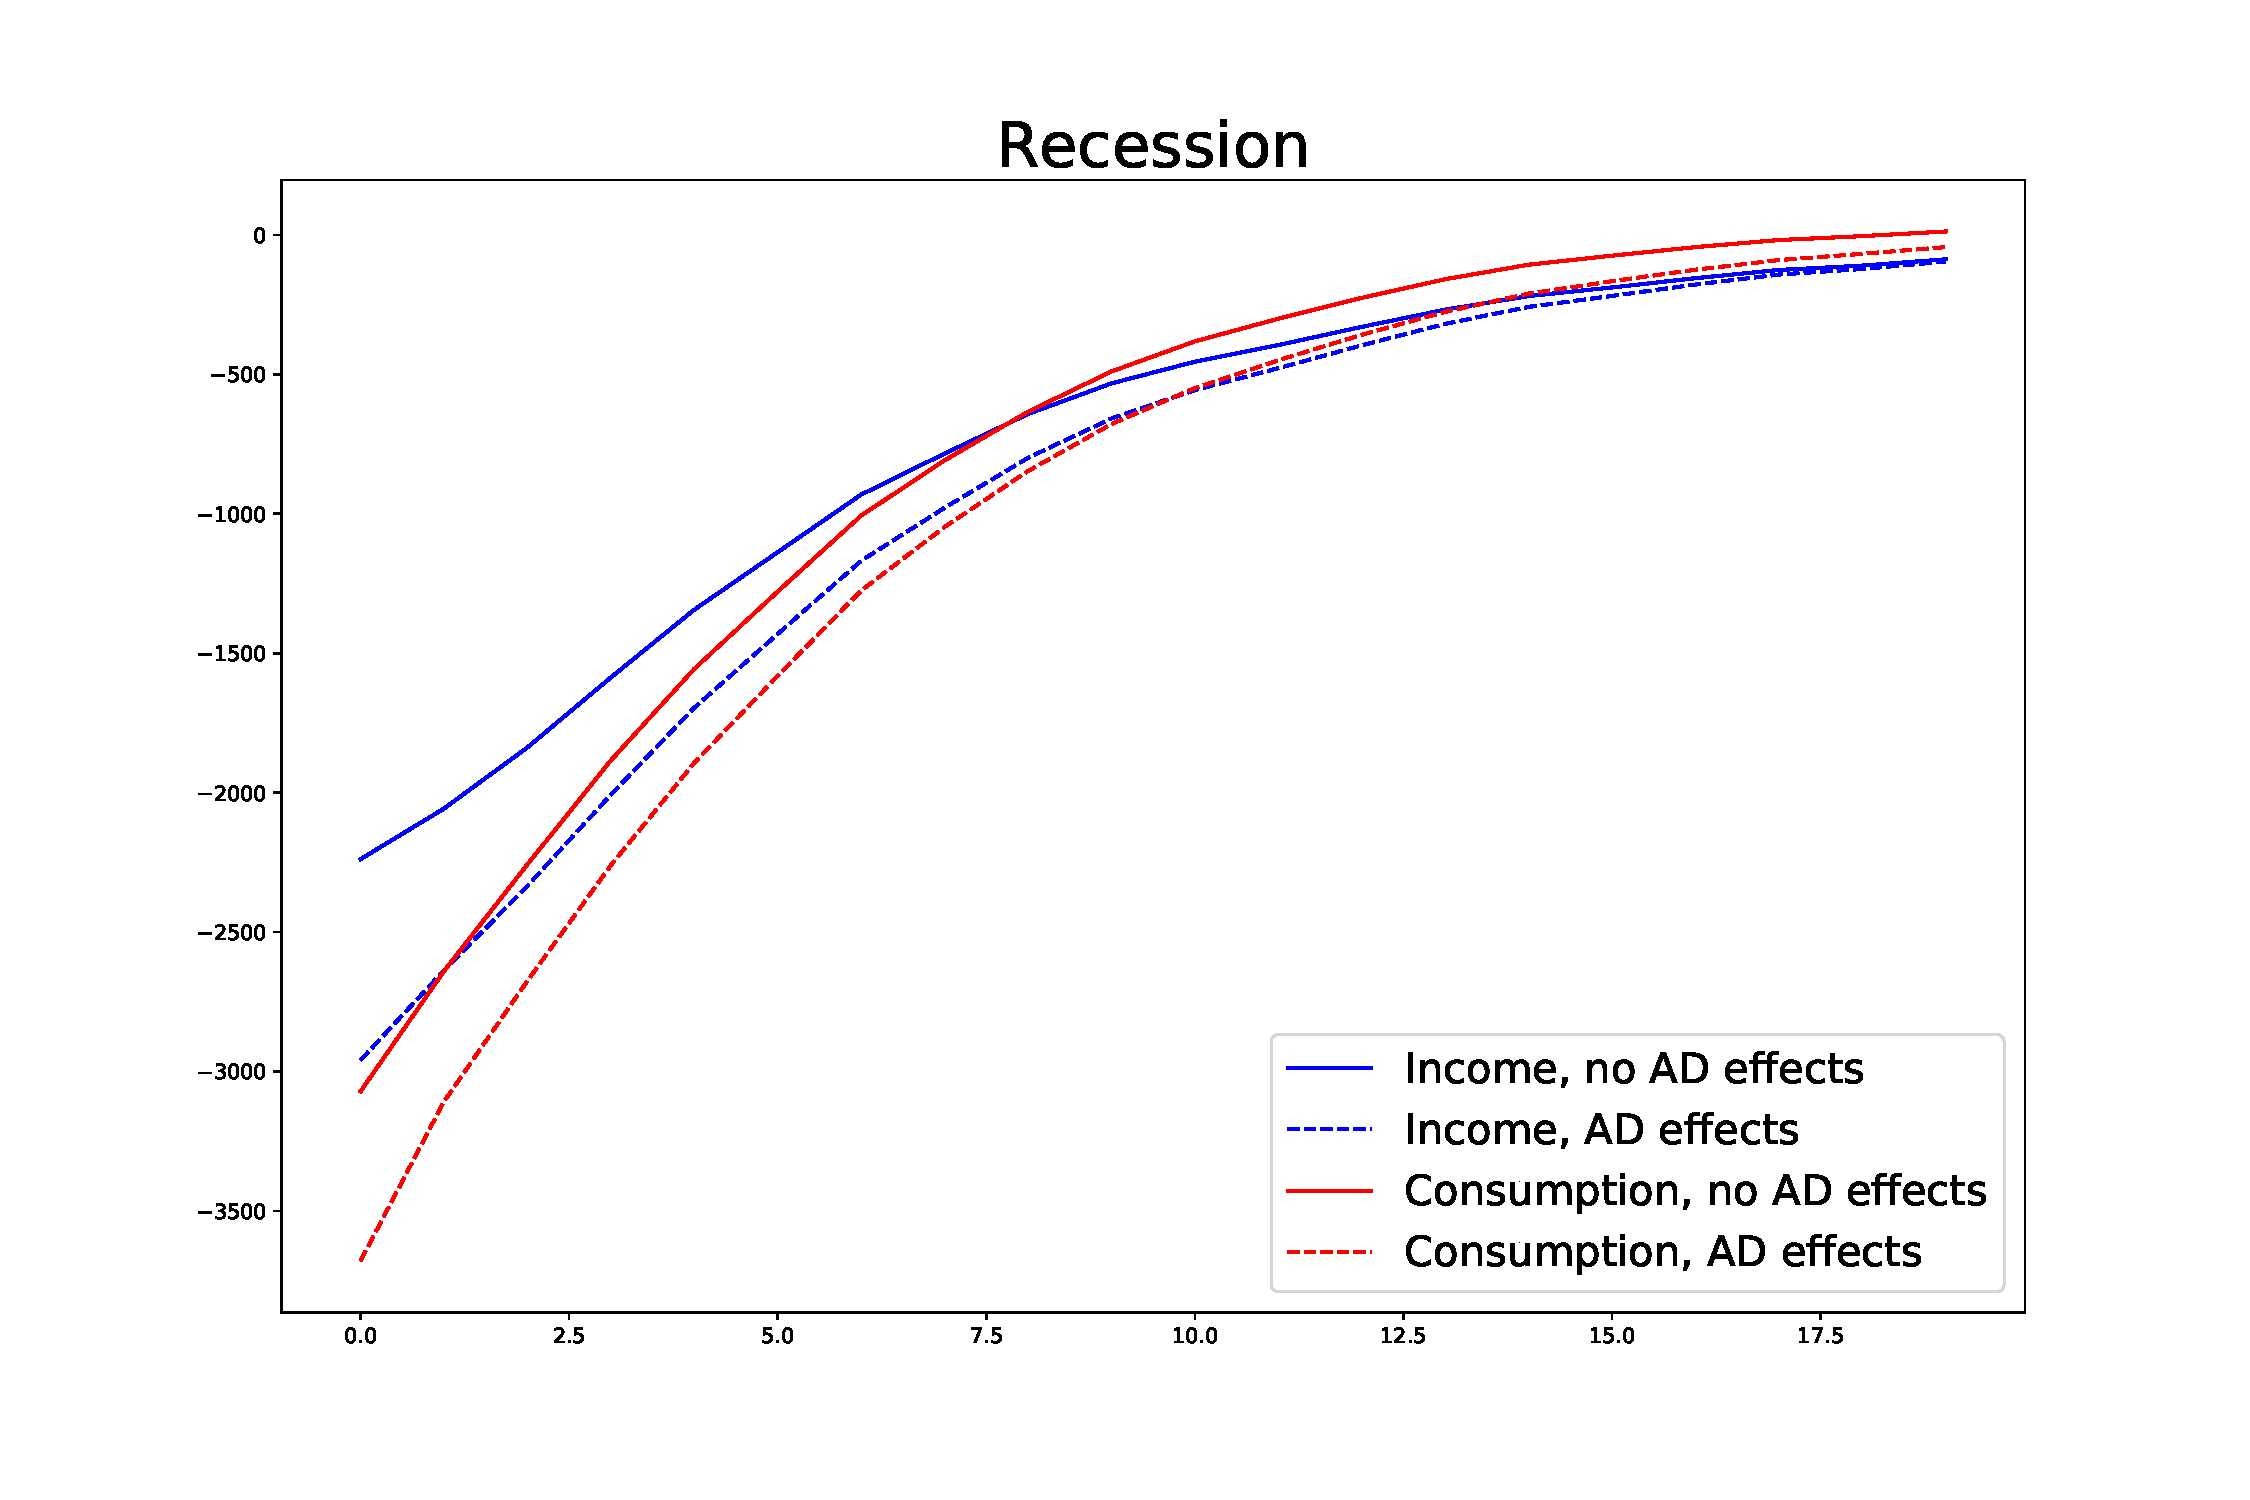
\includegraphics[width=\linewidth]{../recession.pdf}
		\caption{Recession}
		\label{fig:recession}
	\end{centering}
\end{figure}

\FloatBarrier
\subsection{Tax cut}

\begin{itemize}
	\item We consider a payroll tax cut by 2 pp for 8q (deterministic length)
	\item See Figure \ref{fig:taxcut}
	\subitem The tax increases income and consequently pushes up consumption
	\subitem The drop in consumption in 9q is due to the fact that the splurge is applied to income in excess of the baseline income, which drops to zero after the tax cut is reversed. Consumption spending remains elevated for some time after the tax cut due to built up savings. 
	\subitem With aggregate demand effects, the effect on consumption is larger as the increased consumption reinforces consumption through higher income due to higher TFP	
\end{itemize}

\begin{figure} 
	\begin{centering}
		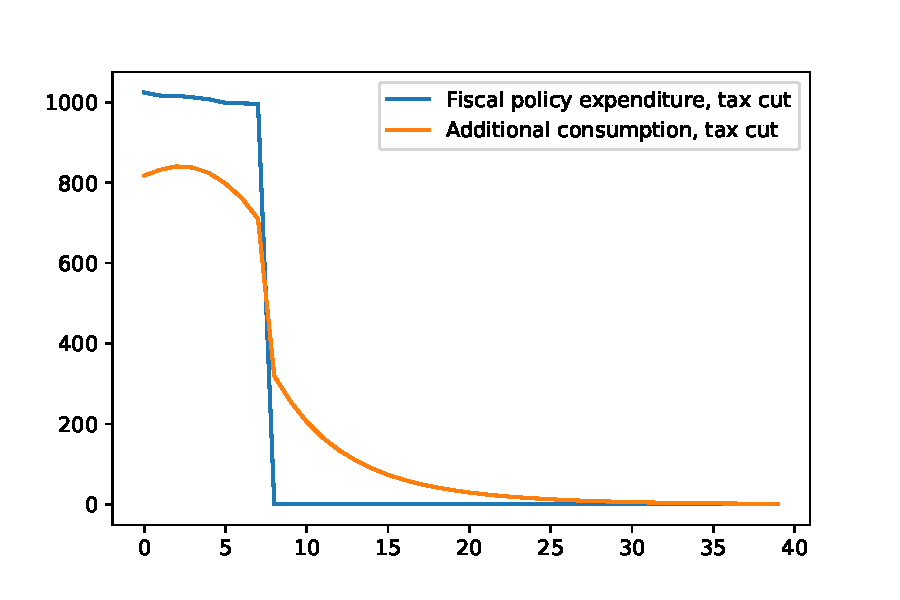
\includegraphics[width=\linewidth]{../tax_cut.pdf}
		\caption{Tax cut}
		\label{fig:taxcut}
	\end{centering}
\end{figure}

\FloatBarrier
\subsection{Tax cut during recession}

\begin{itemize}
	\item We consider a payroll tax cut by 2 pp for 8q (deterministic length) during a recession with an expected length of 6q
	\item See Figure \ref{fig:taxcutrecession}
	\subitem The end of the payroll tax cut induces a second dip in income and consumption
	\subitem In order to measure the role of the aggregate demand effects we need to compare multipliers of the payroll tax cut (i.e. additional stimulus relative to baseline)
\end{itemize}

\begin{figure} 
	\begin{centering}
		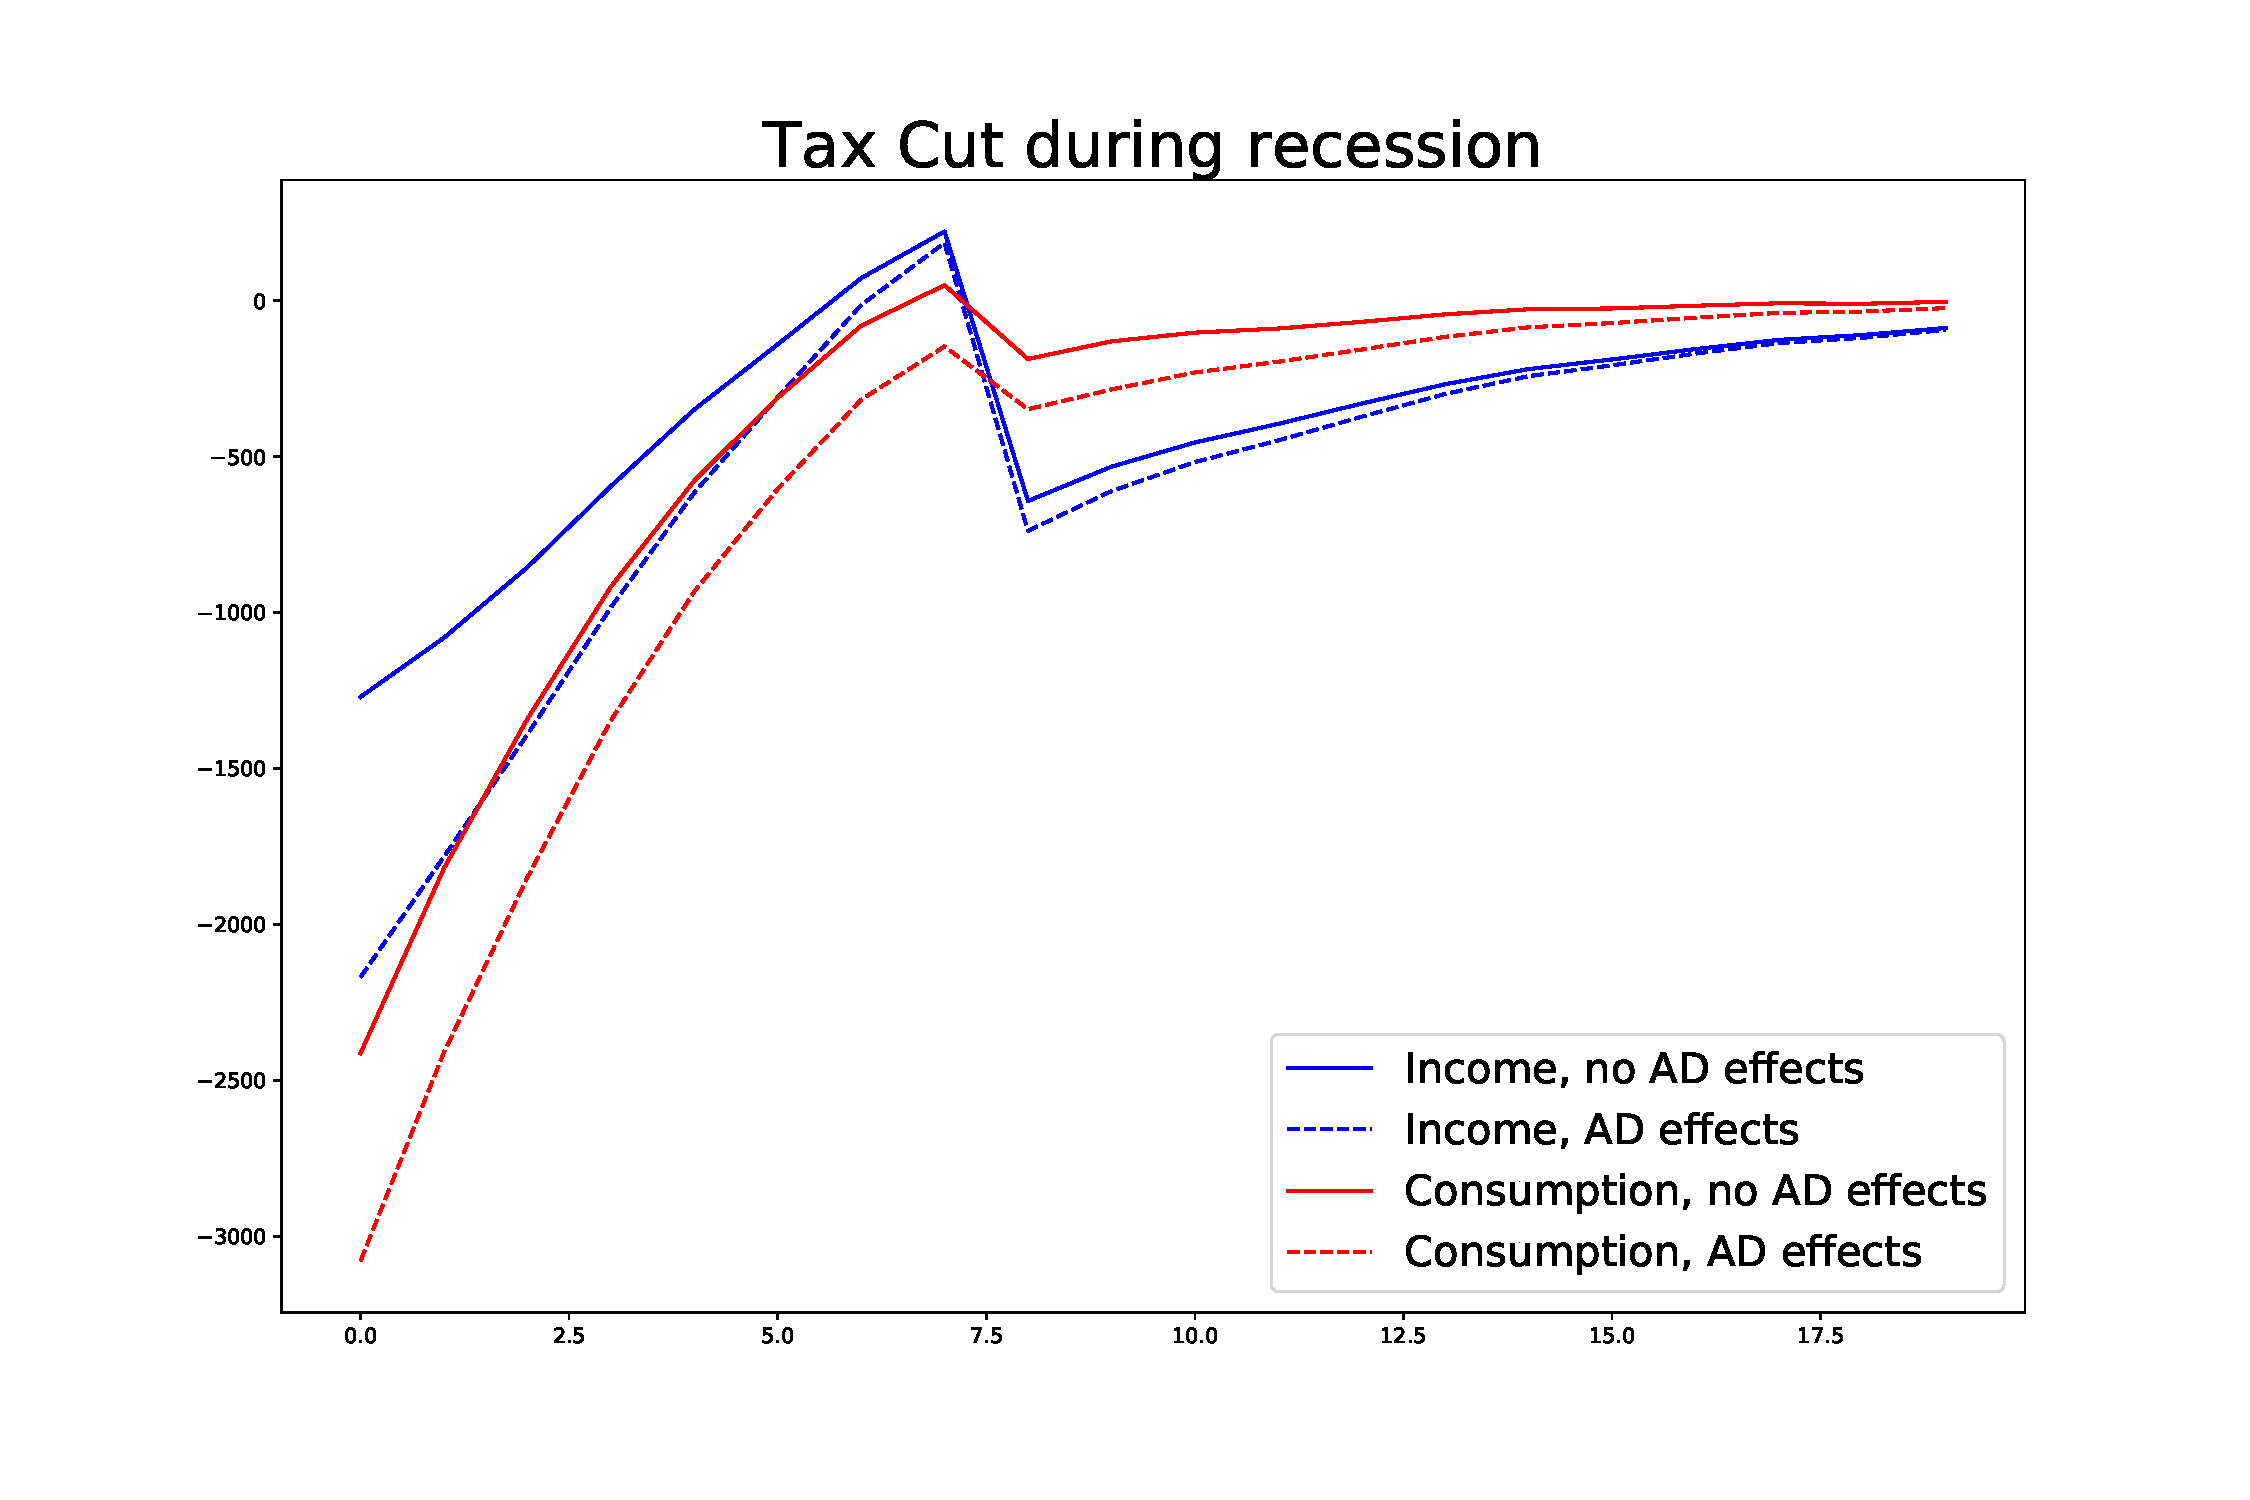
\includegraphics[width=\linewidth]{../taxcut_recession.pdf}
		\caption{Tax cut during a recession}
		\label{fig:taxcutrecession}
	\end{centering}
\end{figure}

\FloatBarrier
\subsection{Tax cut during recession}

\begin{figure} 
	\begin{centering}
		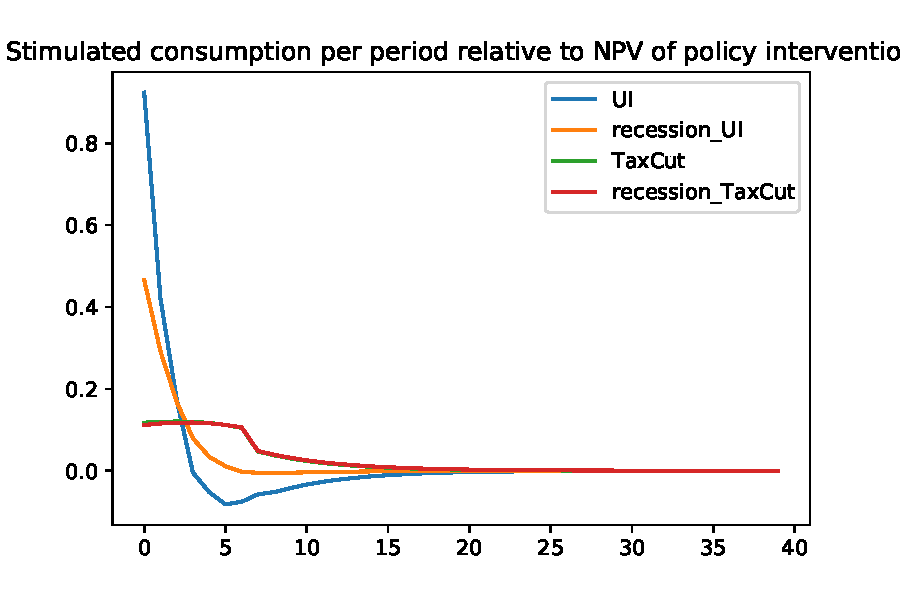
\includegraphics[width=\linewidth]{../stimulated-consumption.pdf}
		\caption{Tax cut during a recession}
		\label{fig:taxcutrecession}
	\end{centering}
\end{figure}


\newpage
\newpage
\section{Old Notes}
\begin{itemize}
	\item What is the research question?
	\item Stimulus checks. Is there a delay - much less so this time around.
	\item Payroll tax cut
	\subitem Is this passed through to workers? Obama stimulus was 2\% ONLY on the employee side
	\subitem Not applicable to the unemployed. 
	\subitem Not applicable to retirees (we don't have lifecycle at the moment).
	\subitem Not applicable to incomes over \$130,000 or there about
	\subitem Is the motivation for a payroll tax cut really consumption stimulus, or is it to encourage more employment (both from worker and employer)
	\item Unemployment benefit extension
	\subitem 26 weeks is standard, Obama increased by 20 weeks
	\item Automatic stabilizer
	\subitem Something like the Sahm rule with stimulus checks going out automatically if ``the three-month moving average of the national unemployment rate (U3) rises by 0.50 percentage points or more relative to its low during the previous 12 months.''
\end{itemize}

General comments
\begin{itemize}
	\item Current focus is on duration of stimulus, rather than targeting specific household characteristics. Is that what we want? There is a argument that stimulus should be ``large and fast'' to get out of a recession, which could come out of a NK type framework. Do we want to make this a focus?
	\item Is a NK framework the correct one here? New Fed consensus statement focuses on employment shortfall, suggesting more of a one-sided model framework.
	\item How do we judge the appropriateness of a policy? Are we going to do welfare analysis?
	\item How do we handle general equilibrium, particularly at the effective lower bound?
\end{itemize}



\end{document}
